\documentclass[14pt,a4paper]{extarticle}
%\documentclass[12pt,a4paper]{article}

\usepackage[utf8]{inputenc}
\usepackage[ukrainian]{babel}


\usepackage{amssymb}
\usepackage{physics}


\usepackage[active]{srcltx}
\usepackage[final]{pdfpages}

\usepackage[hidelinks]{hyperref}

\usepackage{verbatim}
%%%%%%%%%%%%%%%%%%%%%%%%%%%%%%%%%%%%%%%%%%%%%%%%%%%%%%%%%%%%%%%%%%
%\pagestyle{empty}                     %нумерацiя сторiнок i т.д.
\pagestyle{headings}                   %нумерацiя сторiнок вгорi зправа i т.д.
%\renewcommand{\baselinestretch}{1.5}   %мiжстрiчковий інтервал
%\parindent=7.5mm                      %абзацний відступ
 \righthyphenmin=2                     %перенос 2 останніх букв
 \pagenumbering{arabic}
 \tolerance=400
 \mathsurround=2pt
 \hfuzz=1.5pt
%%%%%%%%%%%%%%%%%%%%%%%%%%%%%%%%%%%%%%%%%%%%%%%%%%%%%%%%%%%%%%%%%%
 \hoffset=-0.5cm        %+2.5cm -- вiдступ вiд лiвого краю
 \voffset=-1.5cm        %+2.5cm -- вiдступ зверху
 \oddsidemargin=0.1cm   %ліве поле
 \topmargin=0.1cm       %верхнє поле
 \headheight=0.5cm      %висота верхнього колонтитулу
 \footskip=1cm          %висота нижнього колонтитулу
 \headsep=0.3cm         %відступ від колонт. до тексту
 \textwidth=17cm        %ширина сторінки
 \textheight=25.5cm     %висота сторінки
%%%%%%%%%%%%%%%%%%%%%%%%%%%%%%%%%%%%%%%%%%%%%%%%%%%%%%%%%%%%%%%%%%
 \newcounter{e}
 \setcounter{e}{0}
 \newcommand{\n}{\refstepcounter{e} (\arabic{e})}
 
 \newcounter{pic}
 \setcounter{pic}{0}
 \newcommand{\pic}[1]{\refstepcounter{pic} \vspace{-0.3cm}\textit{Рисунок \arabic{pic}\label{#1}.}}
 
 \newcounter{tabl}
 \setcounter{tabl}{0}
 \newcommand{\tabl}[1]{\refstepcounter{tabl} \vspace{-0.3cm}\textit{Таблиця \arabic{tabl}\label{#1}.}}
 
 \newcounter{dod}
 \setcounter{dod}{0}
 \newcommand{\dod}[1]{\refstepcounter{dod} \textit{Додаток \arabic{dod}\label{#1}.}}
 
% \newcounter{defn}
 %\setcounter{defn}{0}
 %\newcommand{\defn}[1]{\refstepcounter{defn} %\textbf{Означення \arabic{defn}\label{#1}.}}
 
 %\newcounter{theorem}
 %\setcounter{theorem}{0}
 %\newcommand{\theorem}[1]{\refstepcounter{theorem} %\textbf{Теорема \arabic{theorem}\label{#1}.}}
 \newtheorem{theorem}{Теорема}[section]
 \newtheorem{defn}[theorem]{Означення}
 \newtheorem{lemma}[theorem]{Лема}
 
 \newcommand{\proof}{\textit{Доведення. \space}}
% \setcounter{page}{1}
% \setcounter{section}{1}

\numberwithin{equation}{section}
\numberwithin{figure}{section}
%%%%%%%%%%%%%%%%%%%%%%%%%%%%%%%%%%%%%%%%%%%%%%%%%%%%%%%%%%%%%%%%%%
 \newcounter{stali}
 \setcounter{stali}{0}
 \newcommand{\s}{\refstepcounter{stali} \arabic{stali}}

 \newcommand{\st}{C_{\s}}
 \newcommand{\stl}[1]{C_{\s \label{#1}}}

 \newcommand{\cd}{{} $$ \vspace{-0.3cm} $$ {}}
 
 \newcommand{\nb}[2]{\righthyphenmin=#2 #1 \righthyphenmin=2}

%%%%%%%%%%%%%%%%%%%%%%%%%%%%%%%%%%%%%%%%%%%%%%%%%%%%%%%%%%%%%%%%%%
 
 \newcommand{\tabboxl}[2]{\parbox{#1}{\vspace{0.1cm} #2 \vspace{0.1cm} }}
 
 
 \newcommand{\tabboxr}[2]{\parbox{#1}{\vspace{-0.3cm}
 		\begin{flushright} #2 \end{flushright} \vspace{-0.3cm} }}
 
 \newcommand{\tabboxc}[2]{\parbox{#1}{\vspace{-0.3cm}
 		\begin{center} #2 \end{center} \vspace{-0.3cm} }}

 \newcommand{\liml}{\lim\limits}
 \newcommand{\suml}{\sum\limits}
 \newcommand{\intl}{\int\limits}
 
 \newcommand{\inttwopi}{\intl_{0}^{2\pi}}
 
 
 %%%%%%%%%%%%%%%%%%%%%%%%%%%%%%%%%%%%%%%%%%%%%%%%%%%%%%%%%%%%%%%%%%
 % bibliography
 %\usepackage[
 %backend=biber,
 %style=numeric,
 %sorting=none
 %]{biblatex}
 %\addbibresource{resources/bibliography.bibtex}
 %%%%%%%%%%%%%%%%%%%%%%%%%%%%%%%%%%%%%%%%%%%%%%%%%%%%%%%%%%%%%%%%%%

 \begin{document}
	
 %\bibliographystyle{insrt}

 \thispagestyle{empty}

 \begin{center}
	\large
	Міністерство освіти і науки, молоді та спорту України \\
	Львівський національний університет імені Івана Франка \\
	Факультет прикладної математики та інформатики \\
	Кафедра обчислювальної математики
 \end{center}

 \vspace{45pt}

 \vfill

 \begin{center}
	{\Huge{Курсова робота}}\\
	{\large на тему:}
 \end{center}

 \begin{center}\Large
	\textbf{\emph{"Розробка алгоритмів захисту від атак на глибокі нейронні мережі"}}
 \end{center}

 \vfill
 \vskip100pt

 \begin{flushleft}
	\hskip8cm 
	Виконав:
	\\ \hskip8cm 
	студент IV курсу групи ПМп-41
	\\ \hskip8cm
	напрямку підготовки (спеціальності)
	\\ \hskip8cm
	113 -- ``Прикладна математика''
	\\ \hskip8cm
	Бугрій Б.О.
 \end{flushleft}

 \begin{flushleft}
	\hskip8cm 
	Науковий керівник:
	\\ \hskip8cm
	доц. Музичук Ю.М.
 \end{flushleft}

 \vfill

 \begin{center}
	\large
	Львів - 2021
 \end{center}

 \newpage
 \thispagestyle{empty}
 \tableofcontents

 \newpage
 \thispagestyle{empty}
 \addcontentsline{toc}{section}{Вступ}
 \section*{Вступ}
 \begin{center}\end{center}

 \begin{comment}
В останні десятиліття людству, завдяки використанню розумних систем штучного інтелекту, вдалося досягти вражаючих результатів у багатьох сферах повсякденного життя. Яскравими прикладами цього є автомобілі, які здатні долати складні маршрути без жодного людського втручання, програмне забезпечення, яке ставить пацієнтам точні діагнози на основі аналізів та іншої детальної інформації, застосунки для розпізнавання та відтворення мовлення і багато іншого.

Значна частина цих проривів завдячує стрімкому розвитку глибоких нейронних мереж (Deep Neural Networks, DNN), які, в порівнянні з іншими алгоритмами машинного навчання, здатні показувати неймовірні результати на основі великих об'ємів даних, іноді навіть перевершуючи людей. 

Такі типи алгоритмів машинного навчання часто використовують антиінтуїтивні, в порівнянні з смисловим значенням, закономірності стосовно певних характеристик \cite{first-work}. Через це вони є вразливими до різного роду зловмисних модифікацій вхідних даних, які можуть призвести до невірних передбачень. Тому ми не можемо бути впевнені в результатах передбачень моделей на 100\%.
\end{comment}

Сьогодні розумні системи штучного інтелекту є невід'ємною частиною життєдіяльності суспільства. Завдяки таким системам людству вдалося досягти значних результатів у багатьох сферах та галузях, таких як, наприклад, медицина, програмна інженерія, машинобудування та робототехніка.

Зараз найбільш поширеним типом алгоритмів машинного навчання є глибокі нейронні мережі, які здатні знаходити закономірності у великих масивах даних, а результати їх роботи часто перевершують людей. Проте, як показали нещодавні дослідження \cite{first-work}, такі алгоритми часто використовують антиінтуїтивні, в порівнянні з смисловим значенням, закономірності стосовно певних характеристик. Через це нейронні мережі є вразливими до різного роду зловмисних втручань, які можуть призвести до невірних результатів.

Моделі, які показують відмінні результати на звичайних даних, можуть бути легко ошуканими зразками, які лише трохи відрізняються від правильно класифікованих прикладів. Це розкриває фундаментальні недоліки в алгоритмах машинного навчання, які можуть бути використані зловмисниками для заподіяння шкоди, що може вплинути на безпеку технологічних процесів людської життєдіяльності і призвести до катастроф великого маштабу.

%-------------------------------------------------------------------------------
... TODO

Щоб ефективно захиститись від можливих загроз, потрібно знати слабкі місця алгоритмів та стратегії нападу, що використовують зловмисники. Саме тому ми розглянемо деякі підходи до атак на нейронні мережі, знання яких дозволить покращити системи машинного навчання, зробити їх більш стійким до зловмисних втручань.

... TODO






 
 \newpage
 \thispagestyle{empty}
 \section{Опис проблеми}
 \subsection{Постановка задачі}
 %Зменшення множини ошукуючих зразків
 
 Нехай система машинного навчання $M$ на основі зразків $x \in S$ робить передбачення $y$. Тут $S$ -- множина всеможливих зразків-зображень з предметної області, які допустимі для використання моделлю $M$.
 
 % ещ в
 \begin{defn}
 	Зразок $x^{adv} = x + \tau$, $x^{adv} \in S$ називається ошукуючим якщо для достатньо малих збурень $\tau$ виконуються такі умови:  
 	\begin{equation}
	 	M(x) = y_{true}
	\end{equation}
	\begin{equation}
	 	M(x^{adv}) \neq y_{true}
 	\end{equation}
 	де $y_{true}$ - правильне передбачення. 
 \end{defn}
 % норма тау менша за деяку константу
 
 Нашою метою є побудова максимально ефектвної моделі машинного навчання, яка буде менш вразливою до такого типу ошукуючих зразків. 

 Задачу захисту моделі від ошукуючої атаки можна формалізувати наступним чином.
 Нехай $S^{adv}(M) \subset S$ -- множина ошукуючих зразків для моделі $M$. Необхідно знайти модель $M'$ яка є, в певному сенсі, модифікацією оригінальної моделі, таку, що
 \begin{equation}
 	S^{adv}(M') = \emptyset.
 \end{equation}
 Такий ``ідеальний'' випадок є практично неможливим, тому ми будемо використовувати пом'якшений варіант, в якому задовільнятиметься умова
 \begin{equation}
 	n(S^{adv}(M')) < n(S^{adv}(M))
 \end{equation}
 де $n(S)$ --кількість елементів в множині S.
 
 \subsection{Альтернативна постановка задачі}
 %Невеликі зміни зразків не призводять до значних змін результатів
 Модель машинного навчання вважається стійкою до ошукуючих зразків якщо результат передбачення не зміниться при невеликих збуреннях ...
 \subsection{Пов'язані поняття}
 
 \newpage
 \thispagestyle{empty}
 \section{Огляд атак на моделі машинного навчання}

 Нейронні мережі є особливо чутливими до атак на білу скриньку. Отримавши доступ до всіх параметрів, у зловмисників з'являється можливість обчислити точні похідні для функцій (у випадку диференційовності моделі), за допомогою яких виконується класифікація. Тоді під час атаки можна застосувати різні чисельні методи для вирішення конкретної проблеми, що дозволяє досягти дуже високої ефективності згенерованих ошукуючих зразків.
 % Окрім того, складно створити дієві механізми захисту моделі від таких атак, бо зловмисник може врахувати їх при створенні ошукуючих зразків. 

 \begin{center}
	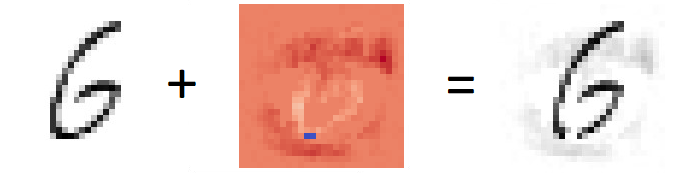
\includegraphics[width=10cm]{../images/six.png}
 \end{center}
 \begin{center}
	\pic{six}
	Початкове зображення класифікується нейронною мережею як ``шість''. Після додавання до нього певного шуму НМ класифікує його як ``п'ять''.
 \end{center}


 Метод швидкого градієнтного спуску є одним з найпростіших методів генерації ошукуючих прикладів. Його застосовують для атак на різні системи машинного навчання, зокрема й на нейронні мережі \cite{explaining-a-e}.

 Основною метою методу є максимізація функції витрат $J$, розглядаючи її як $J(x, y_{true})$, зафіксувавши ваги нейронної мережі. В такому випадку потрібно знайти $x^{adv}$ таке, що виконується нерівність: 

 $$
 J\left(x^{adv}, y_{true}\right)>J\left(x, y_{true}\right)
 \eqno \n \label{convergency}
 $$
 Тоді, згідно з \cite{quarteroni}, ми зможемо знайти розв'язок поставленої задачі. Пошук ошукуючих зразків здійснюємо за формулою:
 $$
 x^{adv} = x + \epsilon {sign}\left(\nabla_x J\left(x, y_{true}\right)\right)
 \eqno \n \label{FGSM}
 $$
 де $\epsilon$ - додатній параметр, який називатимемо \textit{розміром кроку}. Напрямок ${sign}\left(\nabla_x J\left(x, y_{true}\right)\right)$ є \textit{напрямком зростання} для функції $J$.

 Варто зауважити, що метод не гарантує знаходження ошукуючого зразка, бо нерівність (\ref{convergency}) свідчить лише про збільшення функції правдоподібності. Тому в загальному випадку доцільно використовувати ітераційну форму методу. Також можна застосовувати інші методи, такі як \cite{C-and-W}, для того, щоб зменшити розмір шуму $\tau$.

 Більшість реальних систем, які використовують нейронні мережі, не розголошують своїх конфігурацій (як от структура мережі і її ваги), тому атаки, накшталт швидкого градієнтного спуску не так просто застосувати на практиці. В деяких сценаріях зловмисники мають можливість використовувати модель для отримання передбачень на основі власних зразків (як от, наприклад, при використанні  програмних інтерфейсів від Google AI чи Amazon). Запити до мережі  дозволено повторювати необмежену кількість разів і на основі результатів покращувати ошукуючі зразки.

 Тоді є можливість обчислити градієнт наближено, для чого достатньо лише результату класифікації $f(x)$ та відповідного вхідного параметра $x$, як показано в \cite{zoo}. Якщо обчислимо часткові похідні наближено, за формулою

 $$
 \frac{\partial J(\mathbf{x})}{\partial \mathbf{x}_{i}} \approx
 \lim_{h \to 0} \frac{J\left(\mathbf{x}+h e_{i}\right)-J\left(\mathbf{x}-h e_{i}\right)}{2h},
 \eqno \n \label{df-zoo}
 $$
 де $e_i$ - вектор, в якому $i$-тий елемент дорівнює одиниці, а всі решта -- нулю, то зможемо застосувати для атаки на чорну скриньку алгоритми, що використовують похідні для розв'язання задачі оптимізації, такі як швидкий градієнтний спуск.

 При використанні наближених значень похідних в методі швидкого градієнту (\ref{FGSM}) вдається досягти результативності, близької до тої, яку отримуємо під час атак на білу скриньку. Це зумовлено тим, що для ефективної роботи методів достатньо лише знаку градієнту. Те, що значення обчислені з певною похибкою, значним чином не впливає на результат. Недоліком такого сценарію є необхідність виконувати класифікацію значну кількість разів, що займає багато часу та ресурсів і може бути легко виявлено.

 TODO розписати детальніше, можливо поділити на розділи


 \subsection{Атаки на ``відкриті'' нейронні мережі}
 \subsection{Атаки на ``закриті'' нейронні мережі}
 
 \newpage
 \thispagestyle{empty}
 \section{Принципи захисту від ошукуючих атак}
 \subsection{Боротьба з штучно створеним шумом}
 \subsection{Надмірне тренування як причина вразливості}
 
 \newpage
 \thispagestyle{empty}
 \section{Захисне випаровування та його модифікації}
 \subsection{Ідея методу та процес тренування}
 \subsection{Оцінка захисту}
 
 \newpage
 \thispagestyle{empty}
 \section{Методи з гарантованою стійкістю}
 \subsection{Захист PixelDP}
 \subsection{Оцінка захисту}
 
 \newpage
 \thispagestyle{empty}
 \section{Висновок}

 \thispagestyle{empty}
 \addcontentsline{toc}{section}{Література}
 \begin{thebibliography}{99}
	
	\bibitem[1]{first-work}
	\textit{Christian Szegedy, Wojciech Zaremba, Ilya Sutskever, Joan Bruna, Dumitru Erhan, Ian Goodfellow, Rob Fergus} /
	Intriguing properties of neural networks /
	arXiv preprint arXiv:1312.6199 (2014)
	
	\bibitem[2]{explaining-a-e}
	\textit{Ian Goodfellow, Jonathon Shlens, Christian Szegedy} /
	Explaining and Harnessing Adversarial Examples /
	arXiv preprint arXiv:1412.6572 (2014)
	
	\bibitem[3]{quarteroni}
	\textit{Alfio Quarteroni, Riccardo Sacco, Fausto Saleri} /
	Numerical Mathematics / --
	Springer, 2000. --300 p.
	
	\bibitem[4]{black-box-2}
	\textit{Nicolas Papernot, Patrick McDaniel, Ian Goodfellow} /
	Transferability in machine learning: from phenomena to black-box attacks using adversarial samples /
	arXiv preprint arXiv:1605.07277 (2016)
	
	\bibitem[5]{zoo}
	\textit{Pin-Yu Chen, Huan Zhang, Yash Sharma, Jinfeng Yi, Cho-Jui Hsieh} /
	ZOO: Zeroth Order Optimization Based Black-box Attacks to Deep Neural Networks without Training Substitute Models /
	arXiv preprint arXiv:1708.03999 (2017)
	
	\bibitem[6]{C-and-W}
	\textit{Nicholas Carlini, David Wagner} /
	Towards Evaluating the Robustness of Neural Networks /
	arXiv preprint arXiv:1608.04644 (2017)
	
	
 \end{thebibliography}

 \end{document}

